% Chapter 1. N x M integrations versus N + M.
\documentclass[tikz,border=6pt]{standalone}
% Shared look for every TikZ figure in the book.
% Colours match book/preamble.tex exactly. Change both or neither.

\usepackage{tikz}
\usepackage{xcolor}
\usepackage{amsmath}
\IfFileExists{libertinus.sty}{\usepackage[mono=false]{libertinus}}{}
\IfFileExists{inconsolata.sty}{\usepackage[varqu,varl,scaled=0.95]{inconsolata}}{}

\usetikzlibrary{
  arrows.meta, positioning, calc, fit, backgrounds, shapes.geometric,
  shapes.misc, decorations.pathreplacing, decorations.pathmorphing,
  patterns, chains, matrix, shadows.blur
}

\definecolor{ink}{HTML}{15181D}
\definecolor{muted}{HTML}{5B6472}
\definecolor{rule}{HTML}{C9CED6}
\definecolor{wash}{HTML}{F4F5F7}
\definecolor{accent}{HTML}{0F5C8C}
\definecolor{accentsoft}{HTML}{E7F0F6}
\definecolor{warm}{HTML}{B4531A}
\definecolor{warmsoft}{HTML}{FBF0E7}
\definecolor{good}{HTML}{2C6E49}
\definecolor{goodsoft}{HTML}{E9F2EC}
\definecolor{danger}{HTML}{9B2226}
\definecolor{dangersoft}{HTML}{FAECEC}

\tikzset{
  font=\sffamily\small,
  >={Stealth[length=5pt, width=4pt]},
  %
  box/.style={
    draw=rule, line width=0.8pt, fill=wash, rounded corners=2pt,
    inner sep=7pt, align=center, text=ink, minimum height=9mm,
  },
  boxa/.style={box, draw=accent, fill=accentsoft},
  boxg/.style={box, draw=good,   fill=goodsoft},
  boxw/.style={box, draw=warm,   fill=warmsoft},
  boxd/.style={box, draw=danger, fill=dangersoft},
  %
  lane/.style={draw=rule, line width=0.7pt, fill=white, rounded corners=2pt,
               inner sep=6pt, align=center, minimum width=26mm},
  %
  flow/.style={draw=accent, line width=1.0pt, ->},
  flowback/.style={flow, densely dashed},
  flowmuted/.style={draw=muted, line width=0.8pt, ->},
  lifeline/.style={draw=rule, line width=0.7pt, densely dotted},
  %
  lbl/.style={font=\sffamily\scriptsize, text=muted, inner sep=2pt},
  lblink/.style={font=\sffamily\scriptsize, text=ink, inner sep=2pt},
  tag/.style={font=\ttfamily\scriptsize, text=accent, inner sep=2pt,
              fill=white, inner xsep=3pt},
  note/.style={font=\sffamily\scriptsize\itshape, text=muted, align=left},
  %
  band/.style={draw=none, rounded corners=1pt},
  tick/.style={draw=muted, line width=0.6pt},
}

% A horizontal timeline bar segment: \barseg{x0}{x1}{y}{colour}{label}
\newcommand{\barseg}[5]{%
  \fill[#4, rounded corners=1pt] (#1,#3-0.16) rectangle (#2,#3+0.16);
  \node[lbl, text=white, font=\sffamily\scriptsize\bfseries]
       at ({(#1+#2)/2},#3) {#5};
}

\begin{document}
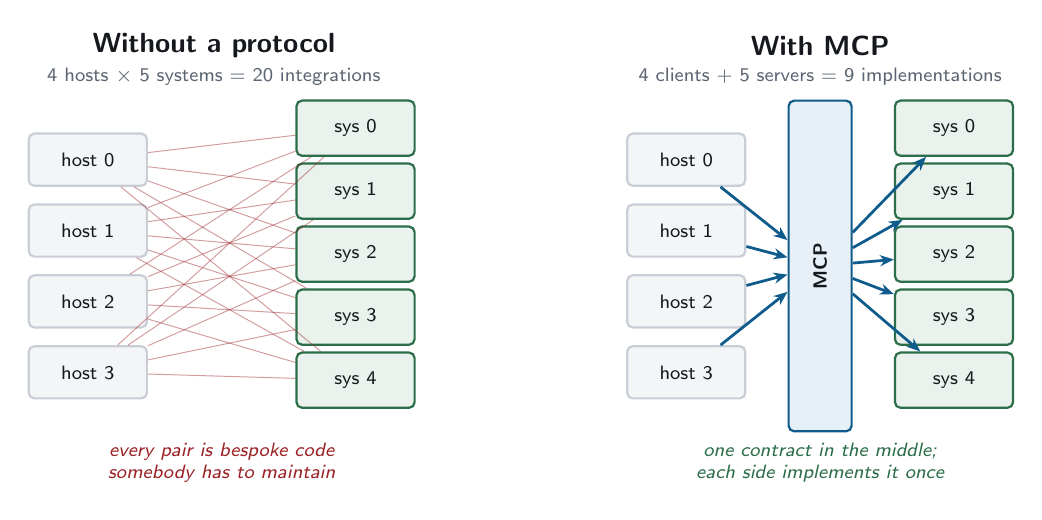
\begin{tikzpicture}[x=1cm, y=1cm]

  % =======================================================================
  % LEFT: the N x M mess
  % =======================================================================
  \begin{scope}[xshift=0cm]
    \node[lblink, font=\sffamily\bfseries] at (1.6,4.15) {Without a protocol};
    \node[lbl] at (1.6,3.75) {4 hosts $\times$ 5 systems = 20 integrations};

    \foreach \i/\y in {0/2.7, 1/1.8, 2/0.9, 3/0.0} {
      \node[box, minimum width=15mm, minimum height=6mm, font=\sffamily\scriptsize]
        (h\i) at (0,\y) {host \i};
    }
    \foreach \j/\y in {0/3.1, 1/2.3, 2/1.5, 3/0.7, 4/-0.1} {
      \node[boxg, minimum width=15mm, minimum height=6mm, font=\sffamily\scriptsize]
        (s\j) at (3.4,\y) {sys \j};
    }
    \foreach \i in {0,1,2,3} {
      \foreach \j in {0,1,2,3,4} {
        \draw[draw=danger, line width=0.35pt, opacity=0.45] (h\i) -- (s\j);
      }
    }
    \node[note, text=danger, align=center] at (1.7,-1.15)
      {every pair is bespoke code\\somebody has to maintain};
  \end{scope}

  % =======================================================================
  % RIGHT: N + M through the protocol
  % =======================================================================
  \begin{scope}[xshift=7.6cm]
    \node[lblink, font=\sffamily\bfseries] at (1.7,4.15) {With MCP};
    \node[lbl] at (1.7,3.75) {4 clients + 5 servers = 9 implementations};

    \foreach \i/\y in {0/2.7, 1/1.8, 2/0.9, 3/0.0} {
      \node[box, minimum width=15mm, minimum height=6mm, font=\sffamily\scriptsize]
        (H\i) at (0,\y) {host \i};
    }
    \foreach \j/\y in {0/3.1, 1/2.3, 2/1.5, 3/0.7, 4/-0.1} {
      \node[boxg, minimum width=15mm, minimum height=6mm, font=\sffamily\scriptsize]
        (S\j) at (3.4,\y) {sys \j};
    }

    % the waist
    \node[boxa, minimum width=8mm, minimum height=42mm, align=center,
          font=\sffamily\scriptsize] (mcp) at (1.7,1.35)
      {\rotatebox{90}{\textbf{MCP}}};

    \foreach \i in {0,1,2,3} { \draw[flow] (H\i) -- (mcp); }
    \foreach \j in {0,1,2,3,4} { \draw[flow] (mcp) -- (S\j); }

    \node[note, text=good, align=center] at (1.7,-1.15)
      {one contract in the middle;\\each side implements it once};
  \end{scope}

\end{tikzpicture}
\end{document}
